% Created 2017-10-26 Thu 18:51
\documentclass[presentation]{beamer}
\usepackage[utf8]{inputenc}
\usepackage[T1]{fontenc}
\usepackage{fixltx2e}
\usepackage{graphicx}
\usepackage{grffile}
\usepackage{longtable}
\usepackage{wrapfig}
\usepackage{rotating}
\usepackage[normalem]{ulem}
\usepackage{amsmath}
\usepackage{textcomp}
\usepackage{amssymb}
\usepackage{capt-of}
\usepackage{hyperref}
\usetheme{default}
\author{weiwu}
\date{\textit{<2017-07-05 Wed>}}
\title{}
\hypersetup{
 pdfauthor={weiwu},
 pdftitle={},
 pdfkeywords={},
 pdfsubject={},
 pdfcreator={Emacs 24.5.1 (Org mode 8.3.4)},
 pdflang={English}}
\begin{document}

\begin{frame}{Outline}
\tableofcontents
\end{frame}

\href{../CS/Python/py4fi/Optimization.html}{PortfolioOptimizationJupyterProgramming}

\href{../CS/Python/py4fi/PortfolioOptimization.html}{PortfolioOptimizationReadMe}

\section{Portfolio Optimization objective functions}
\label{sec:orgheadline1}
\begin{itemize}
\item risk parity portfolios (Roncalli, 2013)
\item Black–Litterman portfolios (Black and Litterman, 1992)
\item log-optimal portfolios (Cover and Ordentlich, 1996)
\item conditional value at risk (cVaR) and coherent risk measures for portfolios (Rockafellar and Uryasev, 2000)
\end{itemize}
\begin{figure}[htb]
\centering
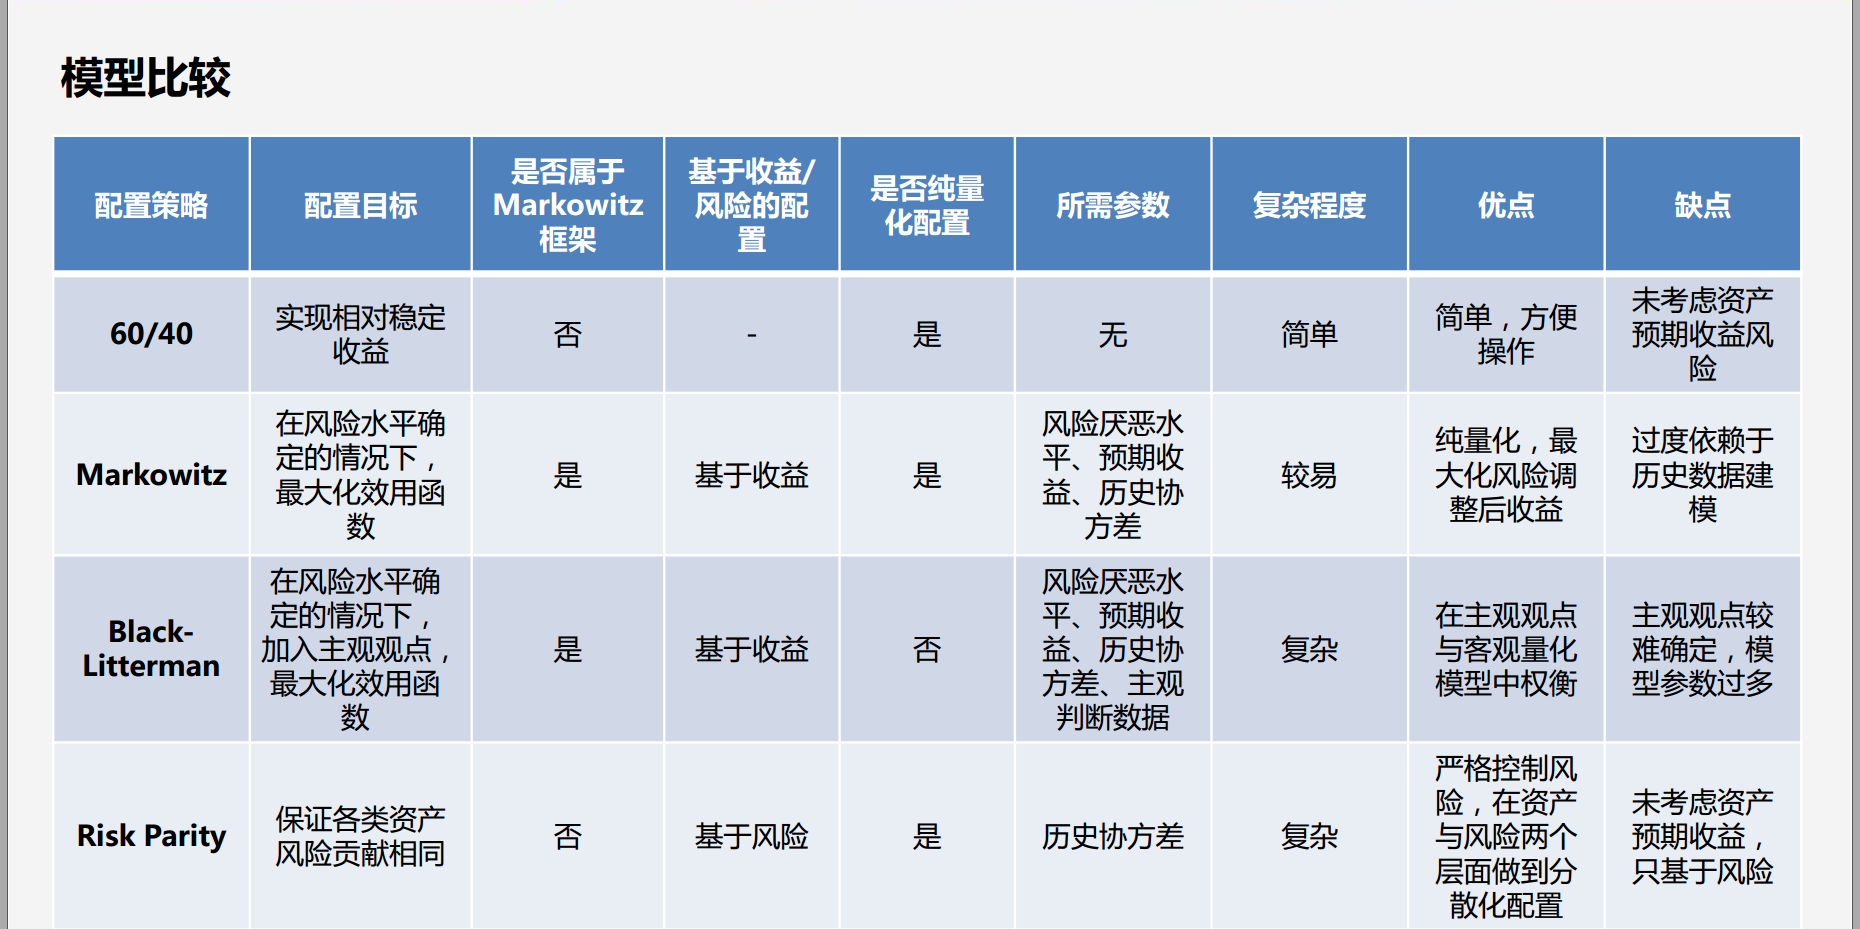
\includegraphics[width=.9\linewidth]{./images/model_comparison.png}
\caption{model comparison}
\end{figure}

\section{Basics}
\label{sec:orgheadline1}
\subsection{Risk aversion parameter}
\label{sec:orgheadline1}
The weight vector that maximizes the expected portfolio growth rate E log(1 + Rtp) (subject to 1T w = 1, w ≥ 0) is called the Kelly optimal portfolio or log-optimal portfolio. Using the quadratic approximation of the logarithm log(1 + a) ≈ a − (1/2)a2 we obtain
\(E[log(1 + Rtp)] ≈ E[Rtp − (1/2)(Rtp)2]
= µT w − (1/2)wT (Σ + µµT )w\),

where µ = Ert and Σ = E(rt−µ)(rt−µ)T are the mean and covariance of the return rt.
\subsection{alpha}
\label{sec:orgheadline1}
Alpha is used to determine by how much the realized return of the portfolio varies from the required return, as determined by CAPM.
\(\alpha = R_{portfolio} - [R_f + (R_m - R_f)\beta]\)
\subsection{Quadratic function}
\label{sec:orgheadline1}
In algebra, a quadratic function, a quadratic polynomial, a polynomial of degree 2, or simply a quadratic, is a polynomial function in one or more variables in which the highest-degree term is of the second degree. For example, a quadratic function in three variables x, y, and z contains exclusively terms x2, y2, z2, xy, xz, yz, x, y, z, and a constant:

\({\displaystyle f(x,y,z)=ax^{2}+by^{2}+cz^{2}+dxy+exz+fyz+gx+hy+iz+j,} f(x,y,z)=ax^{2}+by^{2}+cz^{2}+dxy+exz+fyz+gx+hy+iz+j,\)
with at least one of the coefficients a, b, c, d, e, or f of the second-degree terms being non-zero.

\subsection{Quadratic programming}
\label{sec:orgheadline1}
\begin{itemize}
\item Quadratic programming (QP) is the process of solving a special type of mathematical optimization problem—specifically, a (linearly constrained) quadratic optimization problem, that is, the problem of optimizing (minimizing or maximizing) a quadratic function of several variables subject to linear constraints on these variables. Quadratic programming is a particular type of nonlinear programming.
\end{itemize}
\subsection{Nonlinear programming}
\label{sec:orgheadline1}
the process of solving an optimization problem defined by a system of equalities and inequalities, collectively termed constraints, over a set of unknown real variables, along with an objective function to be maximized or minimized, where some of the constraints or the objective function are nonlinear.
\subsection{Equality constraints}
\label{sec:orgheadline1}
Quadratic programming is particularly simple when Q is positive definite and there are only equality constraints; specifically, the solution process is linear. By using Lagrange multipliers and seeking the extremum of the Lagrangian, it may be readily shown that the solution to the equality constrained problem
\({\text{Minimize}}\quad {\tfrac {1}{2}}\mathbf {x} ^{\mathrm {T} }Q\mathbf {x} +\mathbf {c} ^{\mathrm {T} }\mathbf {x}
{\text{subject to}}\quad E\mathbf {x} =\mathbf {d}\)

is given by the linear system

\({\begin{bmatrix}Q&E^{T}\\E&0\end{bmatrix}}{\begin{bmatrix}\mathbf {x} \\\lambda \end{bmatrix}}={\begin{bmatrix}-\mathbf {c} \\\mathbf {d} \end{bmatrix}}\)
where \({\displaystyle \lambda }\)  is a set of Lagrange multipliers which come out of the solution alongside \({\displaystyle \mathbf {x} }\) .
\subsection{Regime shifts}
\label{sec:orgheadline1}


OLS assumptions:
\begin{itemize}
\item Linear in Parameters
\item Random Sample of n Observations
\item Zero Conditional Mean
\item No Perfect Collinearity
\item Homoskedasticity
\end{itemize}

Pitfall of Modern Portfolio Theory(MPT):
\begin{itemize}
\item It is based on the historical return performance. If the political visk shows up or the fund changes policy or manager, the corporate or the fund performance may change, investor views can't be integrated into the problem.
\end{itemize}

\section{Sparse Markowitz Portfolios}
\label{sec:orgheadline1}

\section{Mean-Reverting Portfolios}
\label{sec:orgheadline1}

\section{Active portfolio management}
\label{sec:orgheadline5}

\subsection{overview}
\label{sec:orgheadline4}
Modern portfolio theory looks at total risk and total return.

The institutional investor cares about active risk and active return.
For that reason, we will concentrate on the more general problem of managing relative to a benchmark.
This focus on active management arises for several \alert{reasons}:

\begin{frame}[label={sec:orgheadline1}]{risk aversion from unknown categories.}
Clients can clump the large number of investment advisers into recognizable categories. With the advisers thus pigeonholed, the client (or consultant) can restrict searches and peer comparisons to pigeons in the same hole.
\end{frame}

\begin{frame}[label={sec:orgheadline2}]{tracking the benchmark}
The benchmark acts as a set of instructions from the fund sponsor, as principal, to the investment manager, as agent. The benchmark defines the manager’s investment neighborhood. Moves away from the benchmark carry substantial investment and business risk.
\end{frame}

\begin{frame}[label={sec:orgheadline3}]{easy tracking for management}
Benchmarks allow the trustee or sponsor to manage the aggregate portfolio without complete knowledge of the holdings of each manager. The sponsor can manage a mix of benchmarks, keeping the “big picture.""
\end{frame}

\section{Exceptional Return, benchmarks and value added}
\label{sec:orgheadline6}
The CAPM provides consensus expected returns. A multiple-factor model can help to control risk.

accurate forecasts of expected return.
a riskfree component (the time premium), a benchmark component\(\beta_n \mu_B\)  (the risk premium), a benchmark timing component\(\beta_n \delta f_B\) (exceptional benchmark return), and an alpha (expected residual return). If Rn is the total return on asset n.
\(E{R_n} = 1 + i_F + \beta_n \mu_B + \beta_n \delta f_B + \alpha_n\)
\begin{itemize}
\item \(\beta_n = \frac{Cov{r_n,r_B}}{Var{r_B}}\)
\item The Risk Premium \(\beta_n \mu_B\)
\end{itemize}
The expected excess return on the benchmark, \(\mu_B\), is usually estimated by analysts as a very long run (70+ years) average (although other estimation methods are common). A number between 3 and 7 percent per annum is reasonable for most equity markets.
\begin{itemize}
\item Exceptional Benchmark return \(\beta_n \Delta f_B\)
\end{itemize}
\(\Delta f_B\) is your measure of that difference between the expected excess return on the benchmark in the near future and the long-run expected excess return.
\begin{itemize}
\item \(\alpha_n\)
\end{itemize}
expected residual return, \$\(\alpha_{\text{n}}\) = E\{\(\Theta_{\text{n}}\)\}.\$
\begin{center}
\begin{tabular}{ll}
parameters & meaning\\
\hline
\(\beta_n\) & the forecast beta of the portfolio versus the benchmark\\
\(r_f\) & risk-free return\\
\(\mu_B\) & benchmark return over the last period(monthly)\\
\(\Delta f_B\) & \(r_p - r_f - \mu_B\)\\
f\(_{\text{b}}\) & \(\displaystyle\sum_{n} h_B(n)E{R_N}-(1+i_F)\)\\
\end{tabular}
\end{center}

\section{Portfolio Construction}
\label{sec:orgheadline16}

\subsection{input:}
\label{sec:orgheadline7}
\begin{itemize}
\item the current portfolio(with certainty)
\item alphas(often unreasonable and subject to hidden biases)
\item covariance estimates(noisy estimates)
\item transactions cost estimates(noisy estimates)
\item an active risk aversion(self-biased)
\end{itemize}
\subsection{constraints}
\label{sec:orgheadline11}
\alert{We can replace any portfolio construction process, regardless of its sophistication, by a process that first refines the alphas and then uses a simple unconstrained mean/variance optimization to determine the active positions.}
\begin{frame}[label={sec:orgheadline8}]{alpha constraint}
\begin{itemize}
\item most institutional portfolio managers do not take short positions and limit the amount of cash in the portfolio.
\item Others may restrict asset coverage because of requirements concerning liquidity, self-dealing, and so on.
\item A manager may require that the portfolio be neutral across economic sectors or industries.
\item The manager may limit individual stock positions to ensure diversification of the active bets.
\item The manager may want to avoid any position based on a forecast of the benchmark portfolio’s performance.
\item portfolio holdings cannot exceed benchmark holdings by more than 5\%.
\end{itemize}
\begin{block}{Scale the Alphas}
\(\alpha=volatility*IC*score\)
\end{block}
\begin{block}{Trim Alpha Outliers}
\end{block}
\begin{block}{Neutralization}
\end{block}
\begin{block}{Risk-Factor-Neutral Alphas}
\end{block}
\begin{block}{For index-tracking portfolios}
\begin{itemize}
\item Take advantage of flexible options for risk control.
\begin{itemize}
\item Minimize the tracking error of your portfolio in the objective or place a hard limit on tracking error using a risk constraint.
\item Use more than one risk model to incorporate several perspectives on risk.
\item Include risk elements that use more than one benchmark or model portfolio.
\end{itemize}
\item Incorporate all the transaction-related costs that impact performance. The transaction cost types available in the optimizer can be used in any combination to accurately reflect overall costs.
\begin{itemize}
\item Capture market impact using non-linear market-impact models (quadratic, 3/2, and 5/3 powers) or a piecewiselinear approximation.
\item Use the fully integrated Goldman Sachs Shortfall Model.
\item Include commissions and brokerage fees using linear costs.
\end{itemize}
\item Place explicit limits on trading activity.
\begin{itemize}
\item Limit overall portfolio turnover or limit turnover of a set of assets.
\item Place asset-specifc limits on trading; for example, limit trade size to a fraction of average daily volume.
\end{itemize}
\item Control portfolio beta using Axioma-provided historical betas, predicted betas computed relative to any benchmark you choose, or betas you supply.
\item Limit the number of names held or traded
\end{itemize}
\end{block}
\begin{block}{For actively managed portfolios…}
In addition to the risk and transaction cost controls available for passive portfolio management, the modeling library contains many options designed to get the most from your alpha signal.
• Augment your risk control using the Alpha Factor. The Alpha Factor compensates for components of your alpha signal that are not included in the risk model, providing more accurate predicted risk estimates.
• Limit risk contributions at the factor or asset level.
• Use Robust Optimization to explicitly incorporate uncertainty in your alpha estimates.
• Incorporate additional tilts in your objective. Tilts can be implemented on any factor, including risk factors, factors from one of Axioma’s factor libraries, or user-supplied factors.
• Prevent small positions and small trades with threshold constraints.
\end{block}
\end{frame}
\begin{frame}[label={sec:orgheadline9}]{risk aversion}
\end{frame}

\begin{frame}[label={sec:orgheadline10}]{transaction cost}
\begin{block}{on stock side}
\begin{itemize}
\item Transactions costs increase with trade size and the desire for quick execution, which help to identify the manager as an informed trader and require increased inventory risk by the liquidity supplier.
\item Transactions costs are difficult to measure. At the same time, accurate estimates of transactions costs, especially distinctions in transactions costs among different stock trades, can significantly affect realized value added.
\item Transactions costs lower value added, but you can often achieve at least 75 percent of the value added with only half the turnover (and half the transactions costs). You can do better by distinguishing stocks by their transactions costs.
\item Trading is itself a portfolio optimization problem, distinct from the portfolio construction problem. Optimal trading can lower transactions costs, though at the expense of additional short-term risk.
\item There are several options for trade implementation, with rules of thumb on which to use when.
\begin{itemize}
\item VWAP.
\item BARRA model.
\end{itemize}
\end{itemize}
\end{block}

\begin{block}{on portfolio side}
\begin{itemize}
\item construct portfolio relative to industry neutral with categories.
\end{itemize}
\end{block}
\end{frame}
\subsection{SCREENS}
\label{sec:orgheadline12}
\begin{itemize}
\item Rank the stocks by alpha.
\item Choose the first 50 stocks (for example).
\item Equal-weight (or capitalization-weight) the stocks.
\begin{itemize}
\item rebalancing:
\begin{itemize}
\item divide the stocks into three categores, top 40, next 60, remaining 100.
\item buy any stocks on the top 40 not in the portfolio.
\item sell any stocks on the bottom 100 in the portfolio.
\item holding any stocks on the middle in the portfolio.
\end{itemize}
\item pros:
\begin{itemize}
\item The screen enhances alphas by concentrating the portfolio in the high-alpha stocks.
\item It strives for risk control by including a sufficient number of stocks (50 in the example) and by weighting them to avoid concentration in any single stock.
\item Transactions costs are limited by controlling turnover through judicious choice of the size of the buy, sell, and hold lists.
\end{itemize}
\item cons:
\begin{itemize}
\item They ignore all information in the alphas apart from the rankings.
\item They do not protect against biases in the alphas.
\end{itemize}
\end{itemize}
\end{itemize}

\subsection{Stratification}
\label{sec:orgheadline13}
\begin{itemize}
\item splitting the list of followed stocks into categories.
\item classify the stocks in each sector by size: big, medium, and small.
\item industry neutral.
\end{itemize}

\subsection{comparison with asset selection and asset allocation}
\label{sec:orgheadline14}
The result is that portfolios constructed using returns-based analysis are very close to mean/variance portfolios, although they require much more effort to construct.
\subsection{solution}
\label{sec:orgheadline15}
\begin{itemize}
\item placing limits on active stock positions.
\item limiting turnover.
\item constraining holdings in certain categories of stocks to match the benchmark holdings.
\end{itemize}
\section{Asset Allocation}
\label{sec:orgheadline19}
Asset allocation comes in several varieties: strategic versus tactical, and domestic versus global.

The process of selecting a target asset allocation is called strategic asset allocation.

The variation in asset allocation around that target is called tactical asset allocation.
\subsection{tactical asset allocation}
\label{sec:orgheadline17}
\begin{itemize}
\item stocks
\item bonds
\item cash
\end{itemize}
\subsection{asset allocation strategies is a three-step process:}
\label{sec:orgheadline18}
\begin{itemize}
\item forecasting returns
\item building portfolios
\item analyzing out-of-sample performance.
\end{itemize}
\section{Black litterman model step-by-step}
\label{sec:orgheadline34}
\subsection{Modern Portfolio Optimization}
\label{sec:orgheadline20}
Markowitz mean-variance optimization:
\(max: \omega\mu - \omega\Sigma\omega'/2\)

Lagrange multiplier solution: \(\omega=(\lambda\Sigma)^{-1}\mu\)

Two most important elements: Expected return \(\mu\), Covariance matrix \(\Sigma\).

\subsection{Problem of mean-variance optimization}
\label{sec:orgheadline21}
\begin{itemize}
\item Extreme long or short positions
\end{itemize}
It could bring extreme long or short positions without constraint(excluding risk exposure constraint, weight constraint).

\begin{itemize}
\item Heavy weight on a small number of assets
\end{itemize}
When subject to a long only constraint, portfolios will concentrate in a relatively small number of assets.

\begin{itemize}
\item Importance of expected return
\end{itemize}
A small increase in the expected return of one of the portfolio's assets can force half of the assets from the portfolio.

\begin{itemize}
\item Lack of investor views
\end{itemize}
Expected return estimate is based on the historical return performance.

If the political risk shows up, macro economy forecast changes, or the fund changes policy or manager, the corporate or the fund performance may change.
Investor views can't be integrated into the problem.

\subsection{Introduction}
\label{sec:orgheadline23}
The Black-Litterman model uses a \alert{Bayesian} approach to combine the subjective views of an investor regarding the expected returns of one or more assets with the market equilibrium vector of expected returns (the prior distribution) to form a new, mixed estimate of expected returns.

prior return distribution -> posterior expected return estimated distribution.

Black–Litterman model is a mathematical model for portfolio allocation developed in 1990 at Goldman Sachs by Fischer Black and Robert Litterman, and published in 1992. It seeks to overcome problems that institutional investors have encountered in applying modern portfolio theory in practice, although the covariances of a few assets can be adequately estimated, \alert{it is difficult to come up with reasonable estimates of expected returns}. The model starts with the equilibrium assumption that the asset allocation of a representative agent should be proportional to the market values of the available assets, and then modifies that to take into account the 'views' (i.e., the specific opinions about asset returns) of the investor in question to arrive at a bespoke asset allocation.

Black–Litterman overcame this problem by not requiring the user to input estimates of expected return; instead it assumes that the initial expected returns are whatever is required so that the equilibrium asset allocation is equal to what we observe in the markets. \alert{The user is only required to state how his assumptions about expected returns differ from the market's and to state his degree of confidence in the alternative assumptions}. From this, the Black–Litterman method computes the desired (mean-variance efficient) asset allocation.

In general, when there are portfolio constraints - for example, when short sales are not allowed.
\begin{itemize}
\item the easiest way to find the optimal portfolio is to use the Black–Litterman model to generate the expected returns for the assets,
\item and then use a mean-variance optimizer to solve the constrained optimization problem.
\end{itemize}

\begin{frame}[label={sec:orgheadline22}]{reverse optimization to mitigate this problem for unconstrainted solution}
\(\Pi = \lambda\Sigma\omega_{mkt}\)
where

\(\Pi\) is the implied excess equilibrium return vector(Nx1 vector);

\(\lambda\) is the risk aversion coefficient, \(\lambda=\frac{E(r)-r_f}{\sigma^2}\);

\(\Sigma\) is the covariance matrix of excess returns(NxN matrix);

\(\omega_{mkt}\) is the market capitalization asset weight(Nx1 vector).

Finally,
\(\omega^* = (\lambda\Sigma)^{-1}\Pi\)
\end{frame}
\subsection{Black-Litterman model and the process of building the required inputs.}
\label{sec:orgheadline27}
\begin{frame}[label={sec:orgheadline24}]{Black-Litterman model}
\begin{block}{Posterior distribution of expected return combining Prior distribution of equilibrium excess return and investor views.}
One of the core assumptions of the model is that the security returns are normally distributed.

\begin{enumerate}
\item Prior equilibrium excess return distribution
\end{enumerate}
Because of this reason during the implementation of model the prior and conditional probabilities are considered to be normally distributed.
\(N~(\Pi, \tau\Sigma)\)

\begin{enumerate}
\item View distribution
\end{enumerate}
\(N~(Q, \Omega)\)

\begin{enumerate}
\item New combined return distribution(Posterior distribution)
\end{enumerate}
Now as the inputs in the Bayes’ rule are normally distributed so will be the posterior probability.
\(N~(E[R], [(\tau\Sigma)^{-1}+(P'\Omega^{-1}P)]^{-1})\)

One can assume different distributions for each of these probabilities and hence create different variants of Black Litterman model.
\end{block}

\begin{block}{Formula}
\(E(R)=[(\tau\Sigma)^{-1}+P'\Omega^{-1}P]^{-1}[(\tau\Sigma)^{-1}\Pi+P'\Omega^{-1}P]\)
where

\(E(R)\)
is the new(posterior) combined return vector(Nx1);

\(\tau\)
is a scalar;

\(\Sigma\)
is the covariance matrix of excess returns(NxN matrix);

\(P\)
is a matrix that identifies the assets involved in the views(KxN);

\(\Omega\)
The level of confidence, expressed as the standard deviation around the expected return of the view. The weaker confidence that is set to a view, the less the view is to affect the portfolio weights.

Is a diagonal covariance matrix of error terms from the expressed views representing the uncertainty in each view(KxK);对第 i 个观点设置信心水平 LCi,根据信心水平和标准刻度因子 CF 来构建观点误差矩阵Ω.

A view has the form \(Q+\epsilon\):
\(\begin{bmatrix}
w1 & 0 & 0\\
0 & ... & 0\\
0 & 0 & w3
\end{bmatrix}\)

\(\Pi\)
is the implied equilibrium return vector(Nx1); Equilibrium is an idealized state in which supply equals demand.
\(\begin{cases}
Litterman & \text {percentage} \\
Satchell and Scowcroft & \text{ equal weight } \\
Thomas Idzorek & \text{ market capital weight }
\end{cases}\)
The relative weighting of each individual asset is proportional to the asset’s market capitalization divided by the total market capitalization of either the outperforming or underperforming assets of that particular view.

It has three factors: 1. the views; 2. the level of condence assigned to each view; 3.the weight-on-views.

The net long positions less the net short positions equal 0.

Thus one can calculate the variance of each individual view portfolio \(p_k\Sigma p'_k\).

\(Q\)
is the view vector(Kx1);
\begin{enumerate}
\item Idzorek method.
\end{enumerate}
\(Q=\begin{bmatrix}
CF/LC_1 &0  &0 \\0
 &...  &0 \\0
 &0  &CF/LC_k
\end{bmatrix}\), where \(CF=P^*\Sigma P^{*t}/(100/50), LC_k=\text {level of confidence of kth view}, P^* \text {1xn vector, sum of each column from P}\)
\end{block}

\begin{block}{Investor views}
Absolute or relative manager views regarding the expected return of some of the assets in the portfolio.

\begin{itemize}
\item absolute view:
\end{itemize}
Asset A will have an absolute excess return of x\%;

\begin{itemize}
\item relative view 1:
\end{itemize}
Asset A will outperform/underperform asset B by xx basis point;

\begin{itemize}
\item relative view 2:
\end{itemize}
Assets A and B will outperform/underperform assets C and D by xx basis points; Equivallently a mini long/short portfolio including A and B vesus a mini short/long portfolio.
\begin{block}{Assessing views}
\begin{block}{Objective}
\begin{itemize}
\item 些财务指标
\end{itemize}
我们考量了其它一些财务指标,如净利润增长率、主营业务收入增长率、净资产收益率等,将各指标进行对比后发现,在我国市场,净利润增长率和主营业务收入增长率等指标非常不稳定、有时具有奇异值,而净资产收益率较为稳定,因此我们在本次实证中使用了净资产收益率作为观点收益,考虑到数据的时效性,我们选用朝阳永续提供的主流券商研究员对行业的一致预期净资产收益率(ROE)数据。

使用上年底的一致预期 ROE 作为观点收益,设置 20\%、 50\%和 80\%三个信心水平, W\(_{\text{mkt}}\) 表示按流通市值权重配置的资产组合.

\begin{itemize}
\item 间接的观点
\end{itemize}
在传统的 B-L 模型中,投资者给出的主观观点是对资产的预期收益,而很多时候投资者可能是一些间接的观点,例如对一些指标的观点(股息率、 EPS、 ROE 等),这些因子可能驱动股价波动。 Wing Cheung 提出了 ABL 模型(Augmented B-L模型),首次将因子模型融入到传统 B-L 模型的框架中,大幅度拓宽了 B-L 模型的适用面。
\end{block}
\begin{block}{Subjective}
\begin{itemize}
\item 分析师主观预期
\end{itemize}
采用行业、个股一致预期( consensus data)是对看法( views)的一个有效构建方式。用个股预期评级综合得分的增长量表示个股预期收益率,具体处理细节是,每一个评分增量(减量)相当于5\%预期收益(或-5\%预期收益)。
\end{block}
\end{block}
\end{block}
\end{frame}
\begin{frame}[label={sec:orgheadline25}]{Inputs}
Input:
\begin{center}
\begin{tabular}{ll}
w & Equilibrium market capitalization weights for each asset.\\
Σ & Matrix of covariances between the assets. Usually computed from historical data.\\
rf & Risk free rate\\
δ & The risk aversion coeffficient of the market portfolio. This can be specified, or can be computed if the investor knows the market return and standard deviation of returns.\\
τ & A measure of the uncertainty of the prior estimate of the mean returns.   Scalar. Proportional to the relative weight given to the implied equilibrium return vector(\(\Pi\)).       Usually between 0.01\textasciitilde{}0.05.\\
\\
\end{tabular}
\end{center}
\end{frame}
\begin{frame}[label={sec:orgheadline26}]{Steps:}
\begin{enumerate}
\item Π = δΣw
\end{enumerate}
Calculate the equilibrium return using reverse optimization.
\(\Pi=\lambda\Sigma\omega_{mkt}\)

Calculate implied market equilibrium returns based on the given benchmark asset allocation weights.
\begin{enumerate}
\item Quantify their uncertainty in the prior by selecting a value for τ.
\end{enumerate}
If the covariance matrix has been generated from historical data, then τ = 1/n is a good place to start.
\begin{enumerate}
\item Formulates their views, specifying P, Ω, and Q.
\end{enumerate}
Given k views and n assets, then P is a k × n matrix where each row sums to 0 (relative view) or 1 (absolute view).
Q is a k × 1 vector of the excess returns for each view.
Ω is a diagonal k × k matrix of the variance of the estimated view mean about the unknown view mean. As a starting point, some authors call for the diagonal values of Ω to be set equal to pTτΣp (where p is the row from P for the specific view). This weights the views the same as the prior estimates.
考虑有K个观点n个资产的例子,此时,P就是k*n矩阵,每一行代表一个观点,Q为K*1矩阵,存放每个观点的超额收益。Ω是k*k对角矩阵,对角线上的每一个元素代表该观点的方差,与对该观点的置信程度成反比:
\(\Omega=(P\Sigma P^T)\tau\)

For example:
\begin{figure}[htb]
\centering
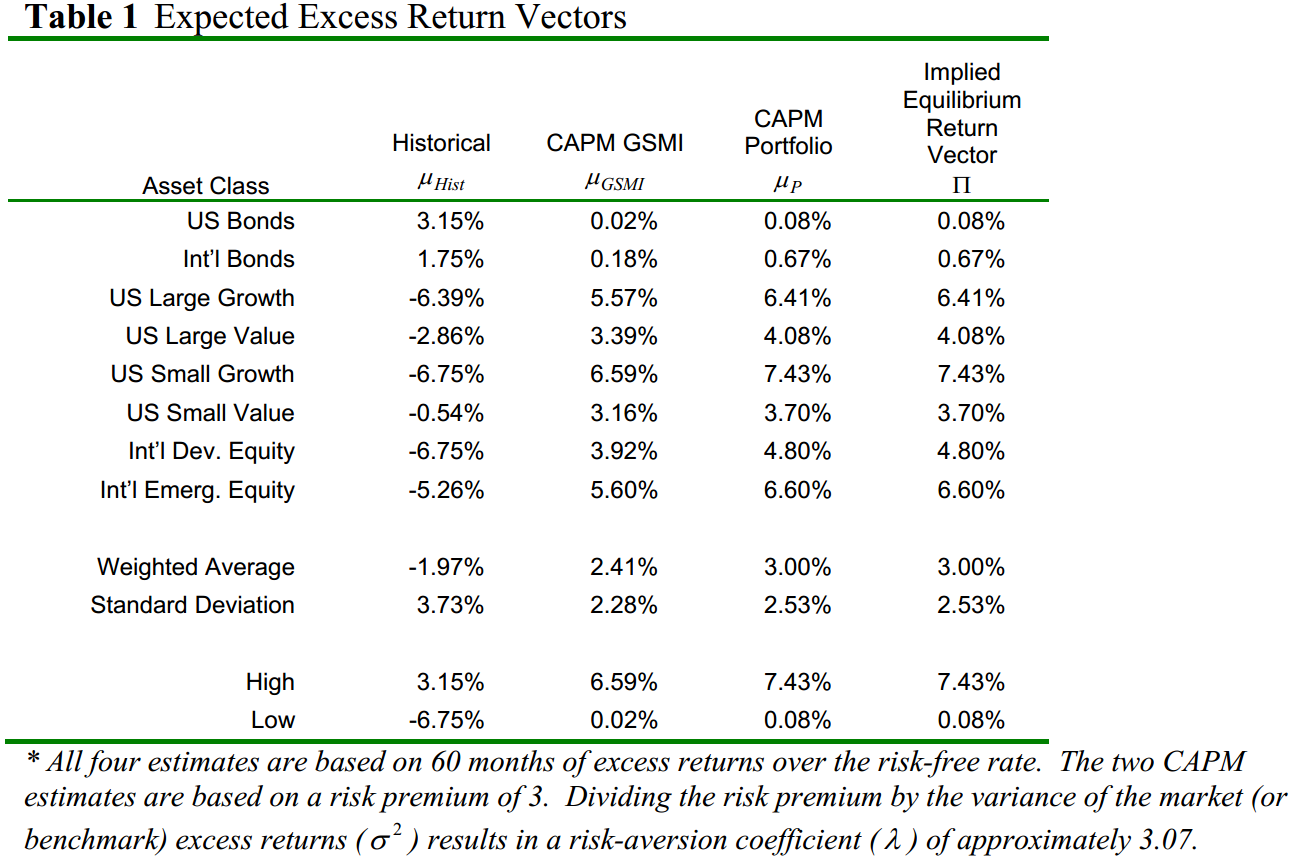
\includegraphics[width=.9\linewidth]{./images/expected_excess_return_vector.png}
\caption{expected\(_{\text{excess}}_{\text{return}}_{\text{vector}}\)}
\end{figure}

View 1: International Developed Equity will have an absolute excess return of 5.25\% (Confidence of View = 25\%).

View 2: International Bonds will outperform US Bonds by 25 basis points (Confidence of View = 50\%).

View 3: US Large Growth and US Small Growth will outperform US Large Value and US Small Value by 2\% (Confidence of View = 65\%).

\(P=\begin{bmatrix}
0 &0  &0  &0  &0  &0  &1  &0 \\
-1 &1  &0  &0  &0  &0  &0  &0 \\
0 &0  &.5  &-.5  &.5  &-.5  &0  &0
\end{bmatrix}\)

\(Q=\begin{bmatrix}
 5.25 \\
 0.25 \\
 2
\end{bmatrix}\)

\begin{enumerate}
\item Compute the posterior estimate of the returns using the following equation.
\end{enumerate}
\(\hat\Pi = \Pi + \tau\Sigma P'(P\tau\Sigma P')^{-1}(Q-P\Pi)\)
\begin{enumerate}
\item Compute the posterior variance of the estimated mean about the unknown mean using the following equation.
\end{enumerate}
\(M=\tau \Sigma - \tau \Sigma P'[P\tau\Sigma P'+\Omega]^{-1}P\tau \Sigma\)
\begin{enumerate}
\item Get the covariance of retujrns about the estimated mean.
\end{enumerate}
Assuming the uncertainty in the estimates is independent of the known covariance of returns about the unknown mean.
\(\Sigma_p = \Sigma + M\)
\begin{enumerate}
\item Compute the portfolio weights for the optimal portfolio on the unconstrained efficient frontier.
\end{enumerate}
\(\hat {\omega}=(\lambda\Sigma_p)^{-1}\hat {\Pi}\)
\end{frame}

\subsection{Implied confidence framework for the views}
\label{sec:orgheadline30}
\(\Omega\), which representing the uncertainty of the views, and \(\tau\) are the most abstract mathematical parameters of this model.

how to specify a probability density function for each view?

\begin{frame}[label={sec:orgheadline28}]{Implied confidence levels}
\(\frac{\hat {\omega} - \omega_{mkt}}{\hat {\omega_{100%}} - \omega_{mkt}}\)
\end{frame}

\begin{frame}[label={sec:orgheadline29}]{An intuitive approach}
\end{frame}

\subsection{Select asset classes}
\label{sec:orgheadline31}
criteria for specifying asset classes are:
\begin{itemize}
\item Assets within an Asset Class should be homogenous.
\item Asset Classes should be mutually exclusive.
\item Asset Classes should be diversifying.
\item All Asset Classes as a group should make up a significant fraction of all investor's wealth.
\item The Asset Class should have the capacity to absorb a significant fraction of the investor's wealth.
\end{itemize}


\begin{itemize}
\item Domestic Equity (can be further sub-divided by value vs growth, or large cap vs small cap).
\item International Equity (can be further divided by developed, emerging, or frontier, or large cap vs small cap, or value vs growth).
\item Domestic Fixed Income (can be further divided by sovereign vs corporate, nominal vs inflation protected, short vs long term, furher sub-divided by issuer or credit rating).
\item International Fixed Income (can be further divided by sovereign vs corporate, nominal vs inflation protected, developed vs emerging, or other distinctions.
\item Real Estate (can be further divided by public vs private, type of real estate holding, loans vs properties, domestic vs international).
\item Commodities (can be further divided by public vs private, by type, e.g. energy vs crops vs metals).
\item Private Equity (can be divided by domestic vs international)
\item Cash or cash equivalents
\end{itemize}

\subsection{Deployment on GS:}
\label{sec:orgheadline32}


\subsection{Pitfall of BLM}
\label{sec:orgheadline33}
\begin{itemize}
\item 非正态分布市场
\end{itemize}
由于 B-L 模型里假设的资产收益都是服从正态分布,这对绝大多数市场来说并不现实, Attilio Meucci 提出了在非正态分布的条件下如何去使用 B-L 模型,并且在对风险的处理中,不再采用传统B-L 模型里的方式,也就是说不再用方差来表示风险,改用 CVAR 等来描述风险,以便能够捕捉到非对称和尾部的风险。

\begin{itemize}
\item 多因子扩展模型
\end{itemize}
在传统的 B-L模型中,投资者给出的主观观点是对资产的预期收益,而很多时候投资者可能是一些间接的观点,例如对一些指标的观点(股息率、 EPS、 ROE 等),这些因子可能驱动股价波动。Wing Cheung 提出了 ABL 模型(Augmented B-L 模型),首次将因子模型融入到传统 B-L 模型的框架中,大幅度拓宽了 B-L 模型的适用面。

\section{NLP}
\label{sec:orgheadline35}
\begin{itemize}
\item Hidden factor model
\item portfolio optimization based on factor model
\item non linear constrain on factor model
\end{itemize}

accounting formula production function, using unit conversion, to do mathematical analysis.

opinions/factors can be used as constraints on factors with hiden factor model.

such factor constraints can be used in Black-Litterman model.
\end{document}